\documentclass[svgnames]{beamer}


% \usepackage{mathtext}
\usepackage[utf8]{inputenc}
\usepackage[english,russian]{babel}
\usepackage{cmap}
\hypersetup{unicode=true}
\graphicspath{{images/}{slides/images}}


\title[CMTA 05] % (optional, use only with long paper titles)
{Text Classification}

\subtitle
{Computational Methods for Text Analysis} % (optional)

\author%[Author, Another] % (optional, use only with lots of authors)
{Pestova Alena}
% - Use the \inst{?} command only if the authors have different
%   affiliation.

\institute%[Universities of Somewhere and Elsewhere] % (optional, but mostly needed)
{HSE Saint-Petersburg}
% - Use the \inst command only if there are several affiliations.
% - Keep it simple, no one is interested in your street address.

\date%[Short Occasion] % (optional)
{04.10.2021}

\subject{natural language processing, text mining}
% This is only inserted into the PDF information catalog. Can be left
% out.


%\AtBeginSubsection[]
%{
%  \begin{frame}<beamer>[plain]{План}
%    \tableofcontents[sectionstyle=show/hide,subsectionstyle=show/shaded/hide]
%  \end{frame}
%}

\newcommand{\tb}[1]{\colorbox{yellow}{#1}\space}
\newcommand{\Sp}[1]{\colorbox{green}{#1}\space}
\newcommand{\Sn}[1]{\colorbox{red}{#1}\space}


\begin{document}

\begin{frame}
  \titlepage
\end{frame}


\begin{frame}[fragile]
  \frametitle{Document-term matrix}
  Terms with the highest DF (document frequency)
  \footnotesize
\begin{verbatim}
Docs вовочк дет класс урок учител учительниц школ
   1      2   0     0    1      0          1    0
   2      2   0     0    0      0          1    0
   3      1   1     0    0      0          1    2
   4      3   1     0    1      0          1    0
   5      3   0     0    0      0          1    0
   6      1   0     0    0      0          1    0
\end{verbatim}
\end{frame}

\begin{frame}
  \frametitle{TF-IDF}
  Term-frequency-inversed document frequency - is a numerical statistic that is intended to reflect how important a word is to a document in a collection or corpus.
  \begin{equation}
    TF \times IDF = tf\log_2\frac{D}{df}
  \end{equation}
  \begin{itemize}
  \item[$tf$]  term frequency - is the relative frequency of term t within document d (raw count of a term in a document / the total number of terms in document)
  \item[$df$] document frequency - the frequency of the word in the collection of documents
  \item $\frac{D}{df}$ inverse document frequency - a measure of how much information the word provides, i.e., if it is common or rare across all documents.
  \item[$D$] the number of all documents in the corpus
  \end{itemize}
\end{frame}


\begin{frame}{Document frequency}
    \begin{itemize}
  \item We can just take the document frequency of each word and put to the matrix
  \item The problem - the length of documents varies greatly
  \item The second problem - not all words characterize the document (stop-words and just common words)

\end{itemize}
\end{frame}


\begin{frame}[fragile]
  \frametitle{TF-IDF}
  Normalization: instead of simple word count (DF) we can weighted frequency  (TF-IDF)
  \footnotesize
\begin{verbatim}
    Terms
Docs    вовочк       дет класс      урок учител учительниц      школ
   1 0.6897996 0.0000000     0 0.4192463      0  0.4022703 0.0000000
   2 0.9197328 0.0000000     0 0.0000000      0  0.5363604 0.0000000
   3 0.2759198 0.4781918     0 0.0000000      0  0.3218162 0.4736512
   4 0.6897996 0.3984932     0 0.2794975      0  0.2681802 0.0000000
   5 1.0346994 0.0000000     0 0.0000000      0  0.4022703 0.0000000
   6 0.6897996 0.0000000     0 0.0000000      0  0.8045405 0.0000000
\end{verbatim}
\end{frame}

\begin{frame}{Vocabulary}
  \begin{itemize}
    \item we may need to limit the vocabulary size (too many features, memory and time complexity, overfitting)
    \item some preprocessing may help (for ex, lemmatization)
    \item cur the vocabulary with some threshold?
  \end{itemize}
\end{frame}

\begin{frame}{Vector space model: summary}
  \begin{itemize}
    \item Text prerpocessing is necessary before building the vectors
    \item We can represent the document as the document-term matrix
    \item We need to think about the vocabulary size (number of columns in this matrix)
    \item Values - just counts of each word in the doc / normalized count
    \item or TF-IDF which helps to reflect how important a word is to a document in a collection or corpus
    \item When we have this matrix we can compare documents (with cosine distance), find similar docs
    \item Or, for ex, we can use this matrix as the data for text classification algorithms
  \end{itemize}
\end{frame}

\begin{frame}{Text Classification}
  Task:
  \begin{itemize}
  \item We have some predefined list of classes
  \item It is necessary to automatically assign a class to each document
  \end{itemize}
\end{frame}

\begin{frame}
  \frametitle{Vectors classification}
  \centering
  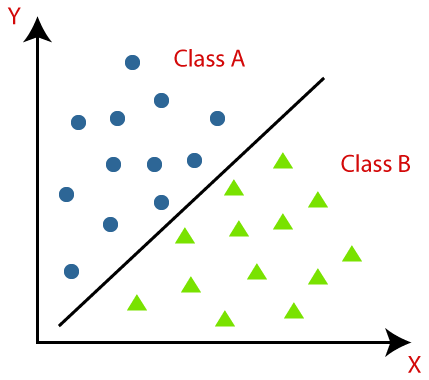
\includegraphics[height=.8\textheight]{classification-algorithm-in-machine-learning}
\end{frame}

\begin{frame}
  \frametitle{Areas of application of the classification in NLP}
  \begin{itemize}
  \item For the whole documents:
    \begin{itemize}
    \item  Defining the language of the text
    \item Defining the topic of the text (from the list of predefined topics)
    \item Sentiment classification (for ex, classifying the review to positive/negative)
    \item Defining the author of the text (from the predefined list)
    \end{itemize}
  \item For the tokens(words):
    \begin{itemize}
    \item part-of-speech tagging (POS-tagging)
    \item Removing homonymy (choosing the meaning of a word)
    \item Named entity recognition
    \item Relations extraction
    \end{itemize}
  \end{itemize}
\end{frame}

\begin{frame}
  \frametitle{Task for ML}
  
Task: learn to predict the properties of an object (text) that are difficult to formalize, but important for a person.

  \begin{itemize}
  \item[target] define the set of the classes (?)
  \item[features] represent the object as a set of features
  \item[model] Based on the statistics of the distribution of properties in texts,
  \item build a model that predicts the labels of new objects (which the model has not yet seen).
    \pause
  \item \alert{PROFIT!}
  \end{itemize}
\end{frame}


\begin{frame}{ML algorithm types}
  \begin{description}
  \item[Supervised learning]

 We have features and target classes - model learns to predict these target classes.

  Example: classification, regression.

  \item[Unsupervised learning]

  No data with target classes, only features.
The model learns to predict based on general assumptions about
    distribution of properties in texts without human preparation
    labeled samples.

    Example: clusterization, topic modelling.

  \end{description}

\end{frame}

\begin{frame}{Classification task}
  Task:
  \begin{itemize}
  \item We have a predefined list of classes
  \item It is necessary to automatically assign each object to one of
    classes
  \item Each object is represented as a set of features.
  \end{itemize}
\end{frame}

\begin{frame}
  \frametitle{new objects classification}
  \centering
  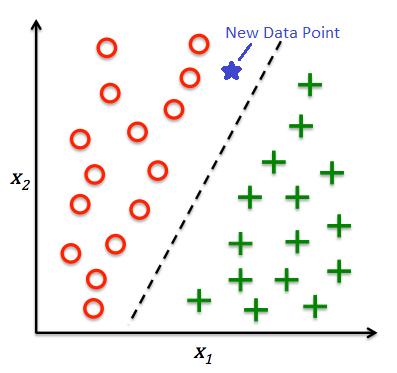
\includegraphics[height=.8\textheight]{new-data-point}
\end{frame}

\begin{frame}{Train-test splitting}
  \begin{description}
    \item[Training Set]
For training of the model.

\item[Validation Set]
 For unbiased evaluation of the model (for tuning hyperparameters on one algorithm)

\item[Test Set]
    For final evaluation of the model.
    
  \end{description}
\end{frame}


\begin{frame}{Train-val-test splitting}
  \begin{itemize}
\item Put aside a part of a dataset (≈ 10 − 20\%) for validation (validation dataset).

\item Train classifier on what is left (training dataset).

\item Optimize hyperparameters (such as tree depth in decision tree, for ex), by the metric on validation
dataset.

\item If we have many hyperparameters, there is a present danger of overfitting to
validation metric. Put aside one more dataset (test dataset).

\item Test your FINAL model on test set.
\end{itemize}

Proportions for train/val/test - smth like 0.7/0.15/0.15, 0.8/0.2/0.2
 \end{frame}

\begin{frame}{Cross-Validation}
  Split to train and test.
  Optimize hyperparameters on train with cross-validation.
  Test the final model on test set.
    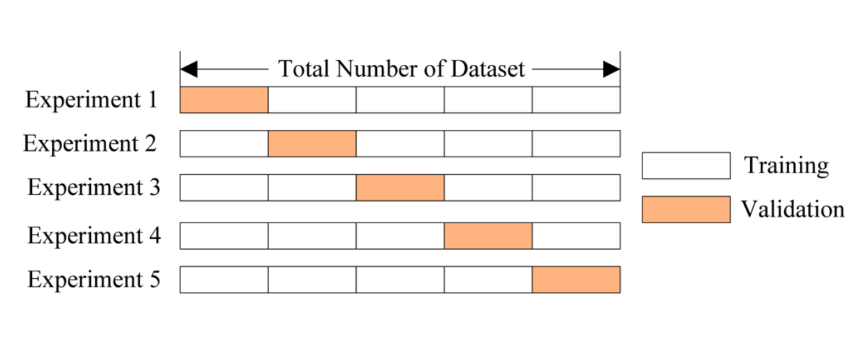
\includegraphics[height=.4\textheight]{cross-validation}
  Better evaluation (all the data is used in train and validation), but slower (is not efficient when we have the big amount ob observations and heavy algorithms)
\end{frame}


\section{Naive Bayes}

\begin{frame}
  \frametitle{Bayes Theorem}
  \only<1>{
    \begin{columns}
      \column{.5\textwidth}
      $$
      P(A \text{and} B) =
      $$

  $$
  P(B)P(A|B) = P(A)P(B|A)
  $$
  \column{.5\textwidth}
  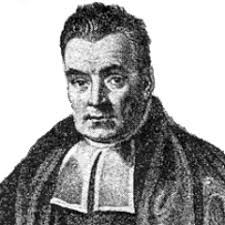
\includegraphics[width=\textwidth]{bayes-himself}
\end{columns}
  }
  \only<2>{
  \begin{equation}
    P(A|B) = \frac{P(B|A)P(A)}{P(B)}
  \end{equation}
  \pause
  \begin{equation}
    posterior = \frac{likelihood \cdot prior}{evidence}
  \end{equation}  
}
\end{frame}

\begin{frame}[standout]
  \begin{itemize}
  \item $P(\text{manager|shy}) = ?$
  \item $P(\text{librarian|shy}) = ?$
  \end{itemize}
\end{frame}

\begin{frame}[standout]
  \begin{itemize}
  \item $P(\text{manager}) = \frac{10 \text{mln}}{80 \text{mln}} = 0.125$
  \item $P(\text{librarian}) = \frac{0,5 \text{mln}}{80
      \text{mln}} = 0.00625$
  \end{itemize}
\end{frame}


\begin{frame}
  \frametitle{Bayes theorem for text classification}
\begin{equation}
    P(\text{label}|\text{features}) = \frac{P(\text{features}|\text{label})P(\text{label})}{P(\text{features})}
  \end{equation}
\end{frame}

\begin{frame}
  \frametitle{Naive Bayes classifier}
  \begin{itemize}
  \item Task:  Having a set of features (E), we need to choose the most probable hypothesis
    (class, H). Denominator Р(E) is a constant and does not affect the results
  $$
   P(\text{label}|\text{features}) \propto P(\text{features}|\text{label}) P(\text{label})
   $$
   \end{itemize}
   \alert{Maximum a posteriory estimation}
\end{frame}

\begin{frame}
  \frametitle{Naive assumption}
\begin{itemize}
 \item Calculate likelihood:
   $$
   P(\text{features}|\text{label}) = 
   $$
 \item \structure{Bayes assumption}: All features are independent:
   $$
   = \prod_{f \in \text{features}} P(f|\text{label})
   $$
 \end{itemize}
\end{frame}

\begin{frame}
  \frametitle{Naive Bayes example}
  % \begin{columns}
  %   \column{.5\textwidth}
    \only<1>{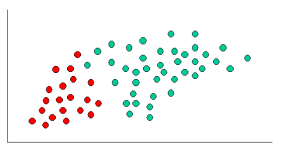
\includegraphics[width=\textwidth]{bayes1}}
  %   \column{.5\textwidth}
\only<2>{
 $$\text{Prior(Green)}\propto \frac{f(\text{Green})}{\text{total}}=\frac{40}{60}$$

 $$\text{Prior(Red)}\propto c\frac{f(\text{Red})}{\text{total}}=\frac{20}{60}$$
}
  % \end{columns}
\end{frame}

\begin{frame}
  \frametitle{Naive Bayes example}
  % \begin{columns}
  %   \column{.5\textwidth}
\only<1>{    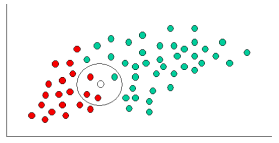
\includegraphics[width=\textwidth]{bayes2}}
    % \column{.5\textwidth}

\only<2>{
    \begin{itemize}
    \item $$\text{Likelihood(X|Green)}\propto \frac{f(\text{Green near X})}{f(\text{Green})}=\frac{1}{40}$$
    \item $$\text{Likelihood(X|Red)}\propto \frac{f(\text{Red near X})}{f(\text{Red})}=\frac{3}{20}$$
    \end{itemize}
}
  % \end{columns}
\only<3>{
  $$
  \text{Posterior(Green|X)} \propto \text{Likelihood(X|Green)} \times
  \text{Prior(Green)} = \frac{4}{6}\times\frac{1}{40}=\frac{1}{60}
  $$

  $$
  \text{Posterior(Red|X)} \propto \text{Likelihood(X|Red)} \times
  \text{Prior(Red)} = \frac{2}{6}\times\frac{3}{20}=\frac{1}{20}
  $$
}

\end{frame}


\begin{frame}
  Naive Bayes is generative classifier:

  \begin{itemize}
  \item build the model of each class
  \item determines the probability that the observed data is generated by the model
    this class
  \end{itemize}
\end{frame}

\begin{frame}{Naive Bayes}
Advantages:
  \begin{itemize}
  \item Suitable for large number of attributes, small training set
  \item Works surprisingly well for a lot of things (and for texts)
  \item Computationally efficient (learns and classifies quickly)
  \end{itemize}
  Disadvantages:
  \begin{itemize}
  \item The independence assumption is wrong.
  \item Null values problem (attribute does not appear in train
    sample) - requires smoothing
  \end{itemize}
\end{frame}

\begin{frame}
  \frametitle{Laplas smoothing}
  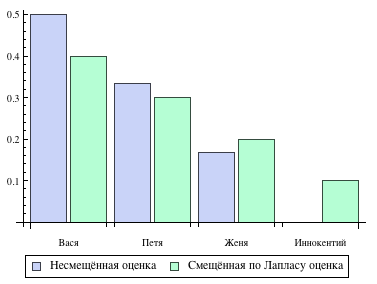
\includegraphics[width=.7\textwidth]{additive-smoothing}
\end{frame}


\begin{frame}[fragile]
  \frametitle{Sparse data problem}
\begin{verbatim}
    Terms
Docs выгребать выгребной выгружать выгрузка выгрызать
   1         0         0         0        0         0
   2         0         0         0        0         0
   3         0         0         0        0         0
   4         0         0         0        0         0
   5         0         0         0        0         0
\end{verbatim}
\end{frame}

\begin{frame}[fragile]
  \frametitle{Curse of dimensionality}
\begin{verbatim}
A document-term matrix (1530 documents, 13322 terms)

Non-/sparse entries: 68859/20313801
Sparsity           : 100%
Maximal term length: 66 
Weighting          : term frequency (tf)
\end{verbatim}
\end{frame}

\begin{frame}
  \frametitle{Hughes phenomenon}
  \centering
  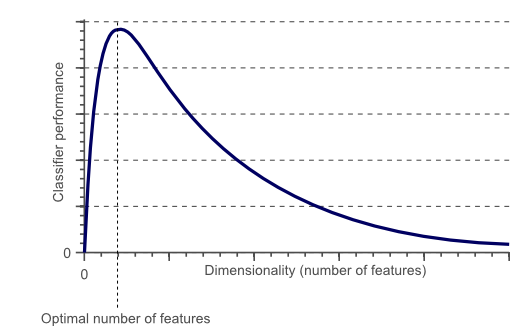
\includegraphics[width=.9\textwidth]{dimensionality_vs_performance}
\end{frame}

\begin{frame}
  \frametitle{Curse of dimensionality}
  \centering
  \includegraphics<1>[width=.6\textwidth]{1Dproblem}
  \includegraphics<2>[width=.6\textwidth]{2Dproblem}
  \includegraphics<3>[width=.6\textwidth]{3Dproblem}
  \includegraphics<4>[width=.6\textwidth]{3Dproblem_separated}
\end{frame}

\begin{frame}
  \frametitle{Overfitting}
  \centering
  \includegraphics<1>[width=.6\textwidth]{overfitting}  
  \includegraphics<2>[width=.6\textwidth]{no_overfitting}  
\end{frame}



\begin{frame}{Dimensionality reduction}
  In machine learning problems that involve learning a "state-of-nature" from a finite number of data samples in a high-dimensional feature space with each feature having a range of possible values,
  typically an enormous amount of training data is required to ensure that there are several samples with each combination of values.
  In an abstract sense, as the number of features or dimensions grows, the amount of data we need to generalize accurately grows exponentially.


  What is more, distances between the points become different from what we except of them. When a measure such as a Euclidean distance is defined using many coordinates, there is little difference in the distances between different pairs of samples.
\end{frame}



\begin{frame}
  \frametitle{Dimensionality reduction}
  \begin{itemize}

\item The matrix of document-terms is very large and sparse
  \item Words that are close in meaning do not necessarily occur in the same
    the same documents:
    \begin{itemize}
    \item synonymy
    \item polysemy
    \item noise
    \end{itemize}
    \pause
  \item We need to reduce the dimension of the matrix (make fewer columns).
  \end{itemize}
\end{frame}

\begin{frame}{Dimensionality reduction}
\begin{itemize}
  \item drop stop-words
  \item lemmatization
  \item Dimensionality reduction algorithms (for ex, PCA)
\end{itemize}
\end{frame}

\section{Evaluating classification algotirhms}
\begin{frame}
  \frametitle{Accuracy}
  \begin{equation}
    \label{eq:a}
    Accuracy = \frac{P}{N}
  \end{equation}
  \begin{itemize}
  \item[$P$] the number of documents where the classifier accepted
    the right decision
  \item[$N$] the size of the training set
  \end{itemize}
\end{frame}


\begin{frame}
  \frametitle{Contingency table}

 Table of correct and incorrect decisions on documents of this class:

  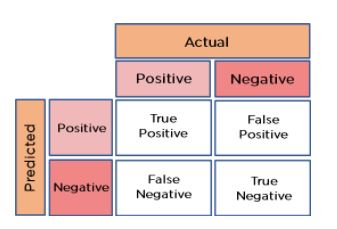
\includegraphics[height=.4\textheight]{confusion-matrix-small}

  \begin{itemize}
  \item[TP] true positive - right prediction of positive class (class 1)
  \item[TN] true negative - right prediction of negative class (class 0)
  \item[FP] false positive - wrong prediction of positive class (true class is 0)
  \item[FN] false negative - wrong prediction of negative class (true class is 1)
  \end{itemize}
\end{frame}

\begin{frame}
  \frametitle{Precision and recall}
  \begin{equation}
    \label{eq:p}
    Precision=\frac{TP}{TP + FP}
  \end{equation}
 Precision is the fraction of relevant instances among the retrieved instances
  \begin{equation}
    \label{eq:r}
    Recall=\frac{TP}{TP + FN}
  \end{equation}
Recall is the fraction of relevant instances that were retrieved.
\end{frame}

\begin{frame}{Precision and recall}
\begin{itemize}
  \item 1
Explain it like fishing with a net. You use a wide net, and catch 80 of 100 total fish in a lake. That’s 80\% recall. But you also get 80 rocks in your net. That means 50\% precision, half of the net’s contents is junk.
\item 2
You could use a smaller net and target one pocket of the lake where there are lots of fish and no rocks, but you might only get 20 of the fish in order to get 0 rocks. That is 20\% recall and 100\% precision.

\end{itemize}
\end{frame}

\begin{frame}
Classification tasks: cancer (0-no cancer, 1-cancer) and spam (0-not spam, 1-spam).

Which metric (precision/recall) is more suitable for each task?

\end{frame}


\begin{frame}
  \frametitle{Confusion matrix}
  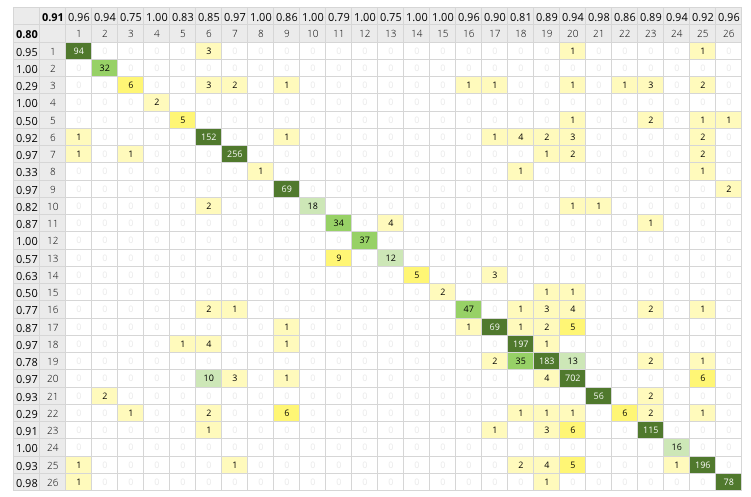
\includegraphics[height=.8\textheight]{confusion-matrix}
\end{frame}


\begin{frame}
  \frametitle{F1-score}
  \begin{equation}
    F_{\alpha} = \frac{(1+\alpha)PR}{\alpha P + R}
  \end{equation}

  \begin{equation}
    F_{1} = \frac{2PR}{P + R}
  \end{equation}  
\end{frame}


\begin{frame}
  \frametitle{Kappa}
  \begin{columns}
    \column{.5\textwidth}
    \begin{equation}
      \kappa = \frac{P_{\mathrm{observed}}-P_{\mathrm{expected}}}{1-P_{\mathrm{expected}}}
    \end{equation}
    \column{.5\textwidth}
    \begin{tabular}{r|ll|r}
     & cats  & dogs \\
      \hline
    cats & 20 & 5 & \alert{25}\\
    dogs & 10 & 15 & \alert{25} \\
    \hline
    & \alert{30} & \alert{20} & 
    \end{tabular}
  \end{columns}
  \only<2>{
    \begin{equation}
      P_{\mathrm{observed}} = (20 + 15)/50 = 0.7
    \end{equation}

    \begin{equation}
      P_{\mathrm{expected}} = ((25*30)/50 + (25*20)/50))/50 = (15 + 10)/50 = 0.5
    \end{equation}
 
    \begin{equation}
      \kappa = \frac{0.7 - 0.5}{1-0.5} = 0.4
    \end{equation}
}
\end{frame}


\begin{frame}{Text Classification: summary}
  \begin{itemize}
    \item Preparing the texts - lemmatization, tokenization, dropping or not dropping smth (important step, affect the classification results)
    \item Prepare the documents as the observations with a set of features (document-term matrix)
    \item Split the data into train-val-test (or just train-test)
    \item Choose the metric for evaluation that is more suitable for your task
    \item (*) if data is very unbalanced in terms of classes - Balancing your data (dropping data/data augmentation techniques)
    \item Choose one/several algorithms, train them on train with different hyperparameters
    \item Choose the best algorithm/algorithms according to your metric
    \item Test final model(s) on test set
    \item (*) interpret results, look at the most important features (words)
  \end{itemize}
\end{frame}

\end{document}
